\documentclass[11pt,a4paper,titlepage]{report}
\usepackage[latin1]{inputenc}
\usepackage{amsmath}
\usepackage{amsfonts}
\usepackage{amssymb}
\usepackage{graphicx}
\usepackage[section]{placeins}
\usepackage{float}
\usepackage{url}
\usepackage{subcaption}
\usepackage[font=small]{caption}
\providecommand{\tightlist}{%
	\setlength{\itemsep}{0pt}\setlength{\parskip}{0pt}}

% todo notes
\usepackage[colorinlistoftodos,prependcaption,textsize=tiny]{todonotes}

\author{MERMET Alexis}
\title{Bachelor Project: Augmenting \textit{pyroomacoustics} with machine learning utilities}
\date{June 8, 2018}

\begin{document}
\maketitle
\tableofcontents
\newpage
%...
\chapter{Introduction}
\section{Objectives of the project}
\hspace*{0.6cm}

\todo{can you look into using bibtex? so that you can cite reference directly in the paper.}

During this project, we want to implement new functionalities to the already existing Python library, \textit{pyroomacoustics}. These functionalities include a wrapper to Google's Speech Commands Dataset\todo{add reference here}, utilities for augmenting  datasets with the already-available room impulse response (RIR) generator, and scripts for evaluating the performance of single and multi-microphone processing for speaker recognition against a pre-trained model.\\
\\
\hspace*{0.6cm}
Before I start, I would like to thank Eric Bezzam for the help he gave me during all the semester, by meeting me every weeks and helping me really quick when I had problem.
I also would like to thank Robin Scheibler who gave me feedback before my presentations even though he is far away from the EPFL and never met me.


\section{What is \textit{pyroomacoustics}?}

\hspace*{0.6cm}
First of all \textit{pyroomacoustics} is a library allowing us to make audio room simulation  and also apply array processing algorithm in Python. Developed by former and current EPFL undergraduate and graduate students, the goal of this library is to aid in ``the rapid development and testing of audio array processing algorithms.'' There are three core components:
\begin{enumerate}
	\tightlist
	\item Object-oriented interface in Python for constructing 2D and 3D simulation scenarios;
	\item A fast C implementation of the image source model for room impulse response (RIR) generation;
	\item Reference implementations of popular algorithms for beamforming, direction finding, and adaptive filtering.
\end{enumerate} 
\hspace*{0.6cm} 
Before the start of this project, we could find five main classes in \textit{pyroomacoustics}: The Room class, the SoundSource class, the MicrophoneArray class, the Beamformer class and the STFT class . Quickly after I began working, Robin Schleiber also added a Dataset class that helped me to start creating a wrapper for Google's Speech Commands Dataset (explained below).\\
\\
\hspace{0.6cm}
With the Room class, you create an object that is a collection of Wall objects, a MicrophoneArray and a list of SoundSource(s). It can be either 2D or 3D.
A SoundSource object has as attributes the location of the source itself and also all of its images sources. In general we create this list directly in the Room object that contains the source.
Finally the MicrophoneArray class consist of an array of microphone locations together with a sampling frequency.
\begin{figure}[h!]
	\centering
	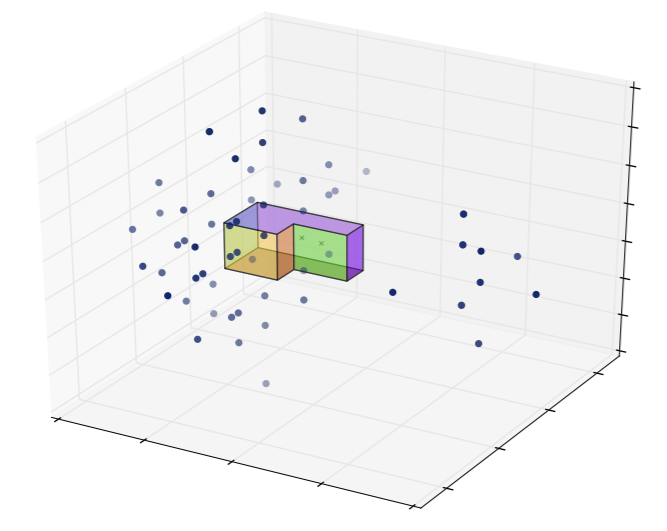
\includegraphics[width=0.7\linewidth]{rapport1}
	\caption[Example of a room in Pyroomacoustic]{Example of a room in Pyroomacoustic.}
\end{figure}

\section{What is TensorFlow?}
\hspace*{0.6cm}
\todo{references!}
As they say on their website, TensorFlow is an``open source software library for high performance numerical computatio". We followed a TensorFlow tutorial called "Simple Audio Recognition" to create the neural networks we used during the all project (we are going to explain how it was created in 2.1). We have also reimplemented some of their functions to be able to label sounds we have modified through processing (see~\ref{sec:label_file}).
\chapter{Theoretical knowledge}
\section{Training the Neural Network}
\hspace*{0.6cm}
In this section we're going to talk about how the neural network was trained. First off all, we download the ``Google's Speech Commands dataset" since we need it to train our network but to test the efficiency of our algorithms. According to the tutorial, this model is considered really simple but is also ``quick to train and easy to understand".\\
\hspace*{0.6cm}
This model works as a convolutional network (in fact this model is similar to the one you can use to do some image recognition). First of all a window of time is defined and the audio signal is converted to an image with the Short Time Fourier Transform (STFT), i.e.\ a spectrogram. This is done by *``grouping the incoming audio samples into short segments and calculating the strength of the frequencies across a set of bands". All the frequency strengths of a given segment will then be treated as a vector of values. These vectors are then ordered according to the time, forming the two-dimensional array known as a ``spectrogram''\\
\begin{figure}[h]
	\centering
	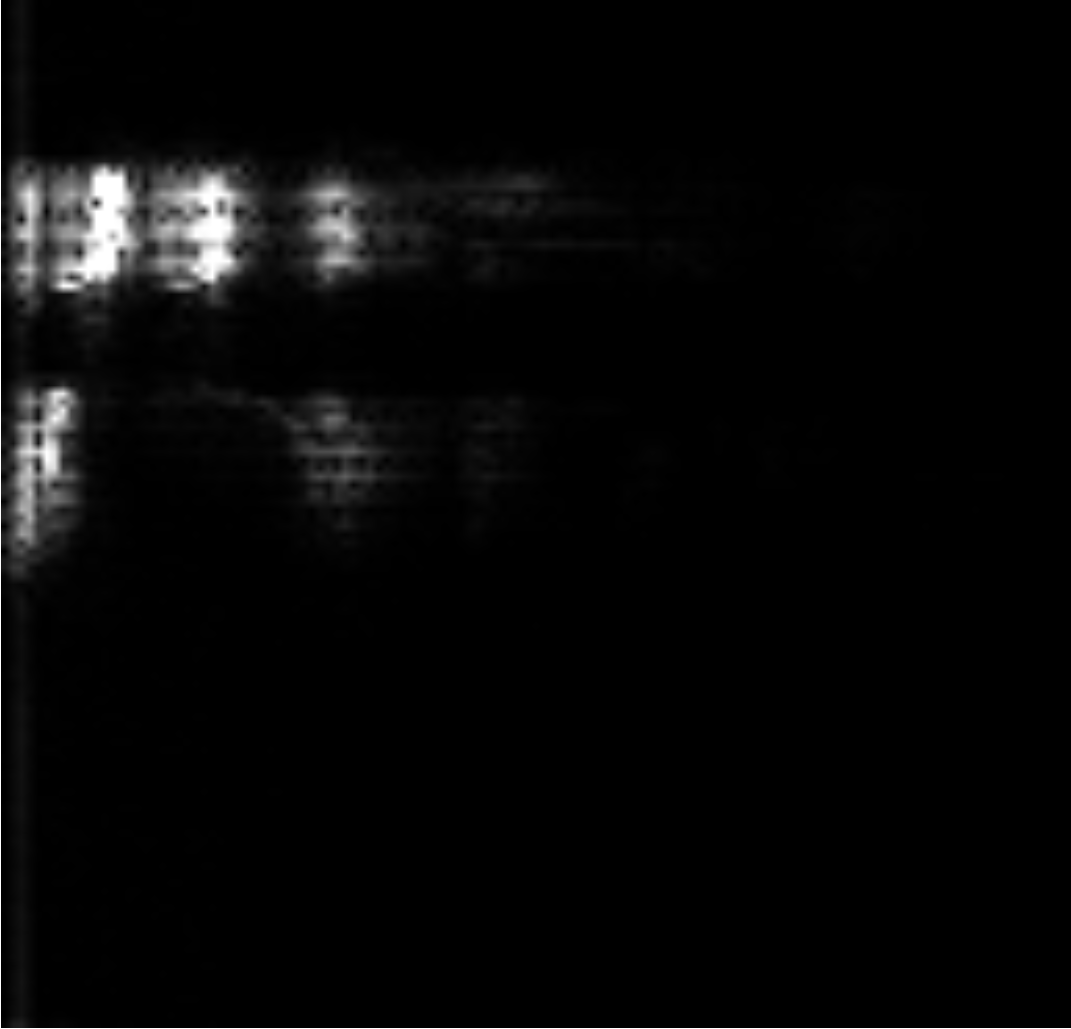
\includegraphics[width=0.7\linewidth]{Rapport2}
	\caption{Spectrogram of one of our sample during the training (image of the TensorFlow website).}
\end{figure}

\hspace*{0.6cm}
In the figure 2.1, time is increasing from top to bottom and frequencies from left to right. We can also see different part of the sound that are probably specific part of it (like a syllable in our case of word).\\
\hspace*{0.6cm}
After our ``image'' is created we can feed it into a multi-layer convolutional neural network (CNN), with a fully-connected layer followed by a softmax at the end. With a large amount of images and associated labels, we can train our network to classify different words. It took between 16h-20h to train the model and we're going to look at its accuracy later on in this report.


\section{The GoogleSpeechCommands Dataset: Basic informations}
\label{sec:google}
\hspace*{0.6cm}
Created by the TensorFlow and AIY teams, the speech command dataset is used to add training and inference in TensorFlow. The dataset contains 65,000 one-second long sound of 30 short words, spoke by "thousands of different people". This dataset is not fixed and will continue to increase with the contribution of users. It is designed to help a user to create his own basic voice recognition interface, with common words like `yes', `no', directions, etc...\\
The different words our system is able to recognize are:

\begin{enumerate}
	\item Yes
	\item No
	\item Up
	\item Down
	\item Left
	\item Right
	\item On
	\item Off
	\item Stop
	\item Go
\end{enumerate}


\section{Signal processing concepts}
\label{sec:Signal processing concepts}
\hspace*{0.6cm}
In this section we're going to talk about one of the most important concept of signal processing we used during this project: the signal-to-noise ratio (SNR). Even though this concept is quite simple and well known, we will talk about it because we it is important in our data augmentation and analysis when we will talk about the implementation (Chapter 4).\\
\hspace*{0.6cm}
First of all, for a single sensor, considering the signal $ y(t) = s(t) + n(t) $, with $ s(t) $ being the sound of interest and $ n(t) $ being the noise, the SNR is defined as the sound power over the noise power.
\begin{equation}
SNR_{sensor} = \dfrac{E[|s(t)^2|]}{E[|n(t)^2|]} = \dfrac{\sigma_{s}^2}{\sigma_{n}^2} 
\end{equation}
with $\sigma_{s}^2$ being the power of the sound of interest and $\sigma_{n}^2$ being the power of the noise.\\
Then if we consider an array of $ M $ sensors and define that the signal received at the sensor $ m $ is $ y_{m}(t) = s_{m}(t) + n_{m}(t) $. We create $ Z(t) $ such that:
\begin{equation}
Z(t) = \sum_{m=0}^{M-1}{w_{m}* y_{m}(t-\Delta_{m})} = Z_{s}(t) + Z_{n}(t) 
\end{equation}
with $ w_{m} $ being the weight corresponding to the signal $ y_{m} $ and $\Delta_{m}$ being a delay that to time-align the separate microphones as the sound does not arrive at the same moment to each sensor.\\
Now we can write the SNR of our beamformed signal $ Z(t) $ as:
\begin{equation}
SNR_{array} = \dfrac{E[|Z_{s}(t)^2|]}{E[|Z_{n}(t)^2|]} = \dfrac{|\sum_{m}w_{m}|^2 \sigma_{s}^2} {\sum_{m}|w_{m}|^2 \sigma_{n}^2} 
\end{equation}
\hspace*{0.6cm}
Finally in this project we don't use the SNR under this form cause it is not really intelligible and easy to use. So we convert it into decibels (dB) such that we now have:
\begin{equation}
SNR_{dB} = 10\log_{10}{\dfrac{\sigma_{s}^2}{\sigma_{n}^2}} = 20\log_{10}{\dfrac{\sigma_{s}}{\sigma_{n}}} 
\end{equation}
\hspace*{3.4cm}(cause $\log_{10}{t^2} = 2\log_{10}{t}$).

\section{Algorithms}
\hspace*{0.6cm}
In this section we are going to talk about the different algorithm we used in this project.
\subsection{Single Noise Channel Removal (SCNR)}
\label{sec:SCNR}
\hspace*{0.6cm}
SCNR is used to suppress the noise, stationary noise in particular. We consider a noisy input signal $ x[n] $ that becomes $ X(k,i) $, with k a specific time and i a frequency, once converted into the frequency domain using the STFT (Short Time Fourier Transform). The noise suppressor removes the noise by applying a time-frequency-varying real-valued gain filter $ G(k,i) $ to $ X(k,i) $. We define this gain filter has follow:
\begin{itemize}
	\tightlist
	\item If there is no noise at a given time and frequency, the gain filter has value 1.
	\item If there is only noise at a given time and frequency, the gain filter has value $ G_{min} $.
	\item If there is a mix of signal and noise at a given time and frequency, the gain filter has a value within $ [G_{min}, 1] $.
\end{itemize}
For this algorithm, an estimation of the noise is needed, we have:
 \[P(k,i) = E[|X(k,i)|^2]  \]
as the estimate of the instantaneous signal + noise, and we need to compute a noise estimate, $ P_{N}(k,i) $. There is two ways to compute it:
\begin{enumerate}
	\tightlist
	\item If the noise is stationary: $ P_{N}(k,i) = \min P(k,i) $ over some past period of time.
	\item Use a voice detector: $ P_{N}(k,i) = P(k,i) $ during a silence period.
\end{enumerate}
In our implementation, we chose the first option, looking back for a fixed number of blocks $ B $:
\begin{equation}
P_{N}(k,i) = \min_{[i- B, \hspace{0.05cm}i]} P(k,i)
\end{equation} 

Now we can define our gain filter such that:
\begin{equation}
G(k,i) = \max[\frac{(P(k,i)- \beta P_{N}(k,i))^\alpha}{P(k,i)^\alpha}, G_{min}]
\end{equation}
where $\beta$ is an overestimation factor, often set to a value larger than one to ensure all noise is suppressed by a factor of $G_{min}$, and the exponent $\alpha$ controls the transition behavior of the gain filter between $G_{min}$ and 1.
\begin{figure}
	\centering
	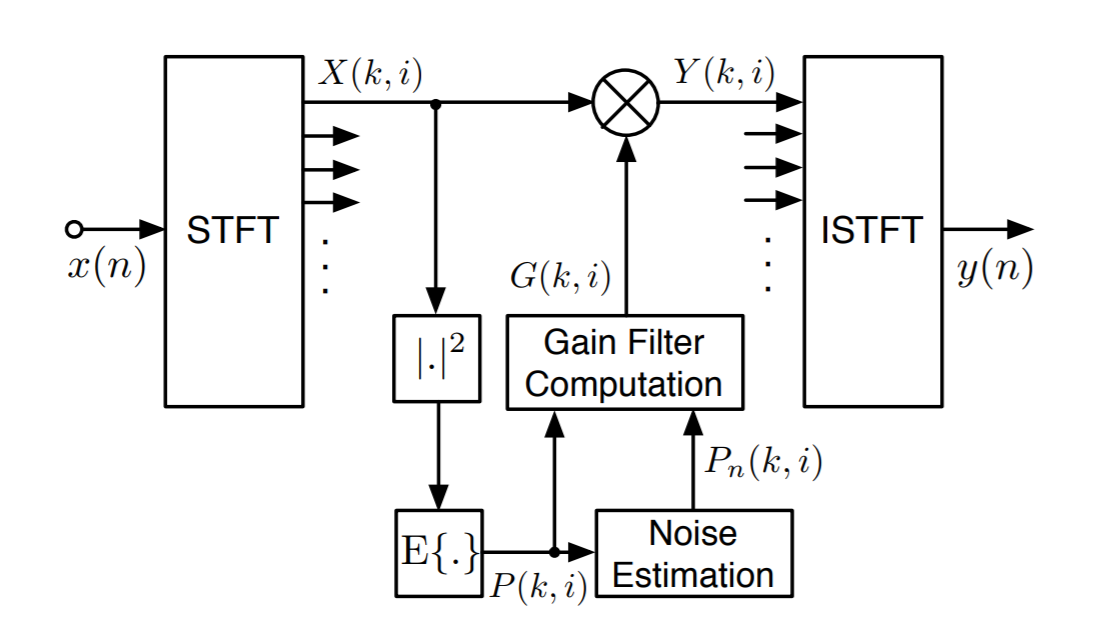
\includegraphics[width=0.7\linewidth]{rapport4}
	\caption{STFT-based stationary noise suppressor (from the Audio Signal Processing and Virtual Acoustics books).}
	\label{fig:rapport4}
\end{figure}

\subsection{Beamforming: Delay and Sum}
\hspace*{0.6cm}
In this section, we are going to talk about one of the most basic \emph{beamforming} algorithm. Beamforming tries to perform an intelligent combination of the sensor signals in order to increase the SNR. Delay and Sum Weights also called Delay And Sum (DAS) looks like what we have saw before hand (see~\ref{sec:Signal processing concepts}). This algorithm takes each individual microphone signal and put all of them in phase by doing a delay correction. Then it add up the different result to obtain a sum signal that is normalized by the number of microphone channels.
If we consider an array of $ M $ sensors and define that the signal received at the sensor $ m $ is $x_m(t)$ then we define $ y(t) $ such that:
\begin{equation}
y(t) = \frac{1}{M}\sum_{m=0}^{M-1}{w_{m}* x_{m}(t-\Delta_{m})}
\end{equation}
with $ w_{m} $ corresponds to the weights, used to improve the quality of the recording, for the $ m^{th} $ signal $ x_{m}  $and $\Delta_{m}$ corresponds to the delay chosen to maximize the array's sensitivity to waves propagating from a particular direction.

\chapter{Implementation}
\section{The GoogleSpeechCommands Dataset}
\hspace*{0.6cm}
The ``GoogleSpeechCommands" dataset wrapper was created as a subclass of the ``Dataset'' class that was already implemented in \textit{pyroomacoustics}. This class will load Google's Speech Commands Dataset in a structure that is convenient to be processed. It has four main attributes: the directory where the dataset is located, the ``basedir". A dictionary whose keys are word in the dataset. The values are the number of occurrences for that particular word in a dictionary called ``size\_by\_samples". A list of subdirectories in ``basedir", where each sound type is the name of a subdirectory, called ``subdirs". And finally ``classes", the list of all sounds, which is the same as the keys of ``size\_by\_samples".\\
\\
\hspace*{0.6cm}
There are multiple functions in this class and we're going to review them quickly to give you a general idea of what is possible with this wrapper.
\\
\begin{enumerate}
	\tightlist
	\item  we have the``init" function that is the builder of our class. When creating a structure containing the Google Speech Command dataset, the user can choose if he wants to download it or not. But he can also choose if he wants to construct just a subset of the all dataset at the start.\\
	\begin{figure}[h!]
		\centering
		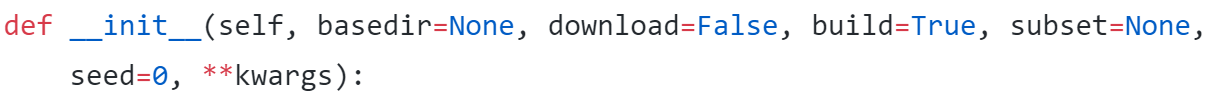
\includegraphics[width=0.95\linewidth]{Rapport5}
		\caption{The "init" function of a GoogleSpeechCommands structure}
		\label{fig:rapport5}
	\end{figure}
	\item The ``build corpus" function that allows the user to build the corpus with some filters, as for example the list of the desired words to be taken from the corpus.\\
	\begin{figure}[h!]
		\centering
		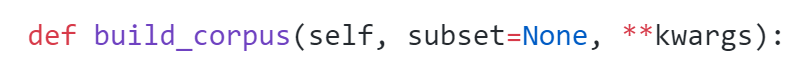
\includegraphics[width=0.7\linewidth]{Rapport6}
		\caption{The "build corpus" function from the wrapper}
		\label{fig:rapport6}
	\end{figure}
	\item The ``filter" function that allows the user to filter the dataset and select samples that match the criterias provided.\\
	\begin{figure}[h!]
		\centering
		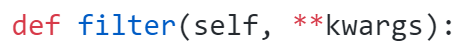
\includegraphics[width=0.4\linewidth]{Rapport7}
		\caption{The "filter" function from the wrapper}
		\label{fig:rapport7}
	\end{figure}
\end{enumerate}
\hspace*{0.6cm}
Now that we talk about the wrapper, we need to present also the ``GoogleSample" class that is inheriting from the class ``AudioSample" created beforehand in \textit{pyroomacoustics}. This class allows the user to create an audio object to print it in a nice way and also to plot the corresponding spectrogram. 

\section{How to label a file?}
\label{sec:label_file}
\hspace*{0.6cm}
In this section, we are going to see how an user can label a file (following the example script available on \textit{pyroomacoustics} called ``how\_to\_label\_a\_file"). This example uses or GoogleSpeechCommand dataset and also the graph we obtained by training TensorFlow neural network.
First of all we rewrote some function of TensorFlow such that we could access the result of labelling. These functions are:
\begin{enumerate}
	\tightlist
	\item load\_graph, that is loading the graph used to label sounds.
	\item load\_labels loads the labels corresponding to the graph (for example: yes, no, etc...)
	\item run\_graph labels a sound and return the prediction (in percentage)
	\item label\_wav, the main function
\end{enumerate}
\hspace*{0.6cm}
The user needs to choose his label file, his graph file. In our example, he can choose one of the word from the list we saw in the ``The GoogleSpeechCommands Dataset: Basic informations" section (see~\ref{sec:google}) and then label it using the ``label\_wav" function in this way:\\
\begin{figure}[h!]
	\centering
	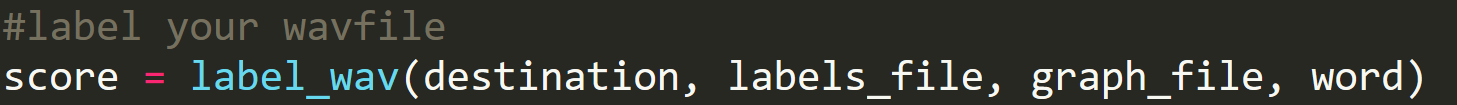
\includegraphics[width=0.7\linewidth]{Rapport8}
	\caption{The labelling function in the \textit{pyroomacoustics} example}
	\label{fig:rapport8}
\end{figure}\\
Here destination represents the directory in which the file to label is kept, labels\_file the label file, graph\_file the graph obtained from TensorFlow and finally word is the sound you except to obtain with this wav file.

\section{How to synthesize noisy signals}
\hspace*{0.6cm}
Now we will learn how to synthesize noisy signals in \textit{pyroomacoustics}. First of all we have implemented, in utils, two function to create noisy signal:
\begin{enumerate}
	\tightlist
	\item modify\_input\_wav
	\item modify\_input\_wav\_multiple\_mics
\end{enumerate}
We will only talk about the second one since the first function is just a special case of the second function. It can be done with the functions taking care of multiple microphones case (but this is less natural to use it in this case).\\
\begin{figure}[h!]
	\centering
	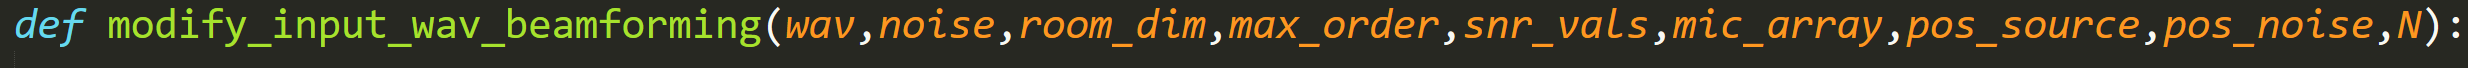
\includegraphics[width=0.7\linewidth]{Rapport9}
	\caption{the modify\_input\_wav\_multiple\_mics functions from \textit{pyroomacoustics}}
	\label{fig:rapport9}
\end{figure}\\
This function will first of all create two rooms, one for the sound source and one for the noise source (we can separate them since the operations we are going to do are linear and the sound independent from the noise) using the dimension, the sound and the noise position given in arguments. After that the room simulation is done, we recover the signals obtained in both rooms. We normalize the noise signal obtained before creating noisy signals for all SNR values given to the function at the start.
\begin{figure}[h!]
	\centering
	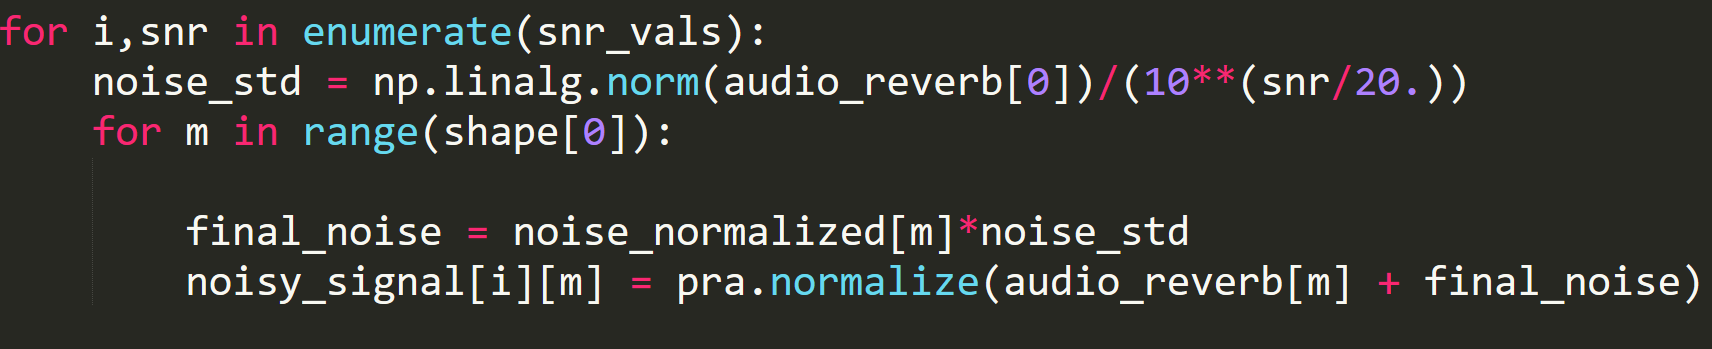
\includegraphics[width=0.7\linewidth]{Rapport10}
	\caption{How to synthesize the noisy signal for each SNR value}
	\label{fig:rapport10}
\end{figure}\\
In the figure above, we compute the noisy signal corresponding to each SNR value. The new noise is obtained by multiplying the normalized noise by a coefficient corresponding to a precise SNR value. We obtain this coefficient from the formula for the SNR (see~\ref{sec:Signal processing concepts}).
\begin{equation}
SNR_{dB} = 20\log_{10}{\dfrac{\sigma_{s}}{\sigma_{n}}} \Leftrightarrow \dfrac{SNR_{dB}}{20} = \log_{10}{\dfrac{\sigma_{s}}{\sigma_{n}}} \Leftrightarrow 10^{\dfrac{SNR_{dB}}{20}}
\end{equation}
\begin{equation}
\Leftrightarrow 10^{\dfrac{SNR_{dB}}{20}} = \dfrac{\sigma_{s}}{\sigma_{n}}
\end{equation}
\begin{equation}
\Leftrightarrow \dfrac{\sigma_{s}}{10^{\dfrac{SNR_{dB}}{20}}} = \sigma_{n}
\end{equation}
with $\sigma_{n}$ being the square root of the noise's power and also the coefficient we are looking for. This coefficient obtained we can compute the new noisy signal , y(t) such that:
\begin{equation}
y(t) = normalized(x(t) + \sigma_{n} * normalized(n(t)) )
\end{equation}
with x(t) the sound signal and n(t) the noise signal.\\
\hspace*{0.6cm}
You can see an example of how to use this function in \textit{pyroomacoustics}. It is called ``how\_to\_synthesize\_a\_signal". In this example, for a word from the GooglepeechCommands dataset (``no") and an SNR of 20, we obtained the following new noisy signal:
\begin{figure}[h!]
	\centering
	\begin{subfigure}{.5\textwidth}
		\centering
		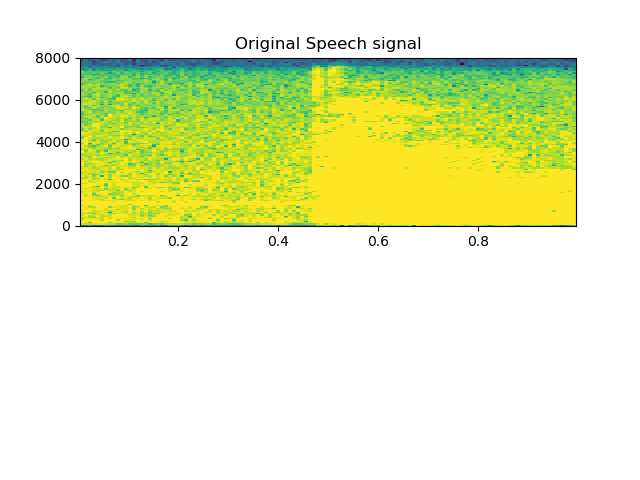
\includegraphics[width=0.91\linewidth]{rapport12}
		\caption{original input signal's spectrogram}
		\label{fig:sub1}
	\end{subfigure}%
	\begin{subfigure}{.5\textwidth}
		\centering
		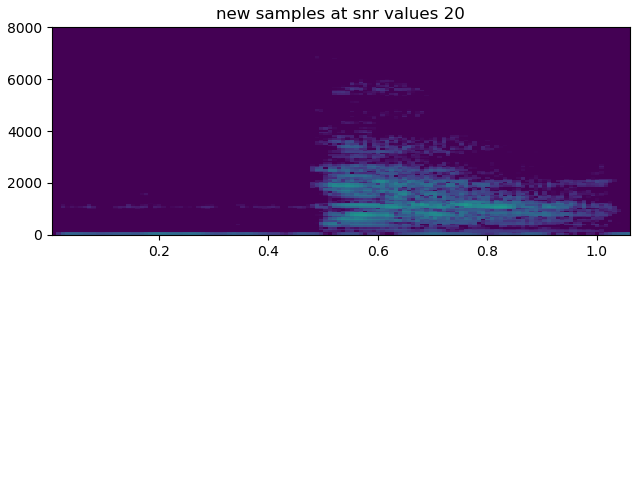
\includegraphics[width=0.91\linewidth]{rapport13}
		\caption{A noisy signal's spectrogram}
		\label{fig:sub2}
	\end{subfigure}
	\caption{original input signal's spectrogram compared to new noisy signal's spectrogram }
	\label{fig:rapport11}
\end{figure}
\section{The algorithms}
\hspace*{0.6cm}
We have implemented one algorithm ourself in this project, the Single Noise Channel Removal (SCNR). The Delay and Sum (DAS) was already implemented in the package with lots of other beamforming algorithm far more efficient that we haven't used.\\
You can see how we implemented it in figure 3.8 however we will explain how we did it.\\
First of all we create an STFT object that allow us to compute short time Fourier transform and to use it in an easy and efficient way. We prepare also an array that will contain all of our processed audio at the end.
Then we implement the algorithm that we run for each SNR values given by the user in this case (example called ``analyse\_improvement\_of\_single\_noise\_channel\_removal" in \textit{pyroomacoustics}). We set a counter n to 0 at the start of the algorithm. It tells us in which chunk of the STFT we are at a given moment. After that, we enter in the while loop where we use the STFT object to our advantage. With it we can compute easily the STFT of our input signal (a noisy signal). Then we fill our matrix containing all the previous signal's power estimation and we select its minimum value as our noise's power estimation. Having this estimation we can now compute the value of our filter, called mask in the figure, using the formula (2.6) (see~\ref{sec:SCNR}). Finally we have to update our matrix containing the powers and our counter n before repeating the actions above.

\begin{figure}
	\centering
	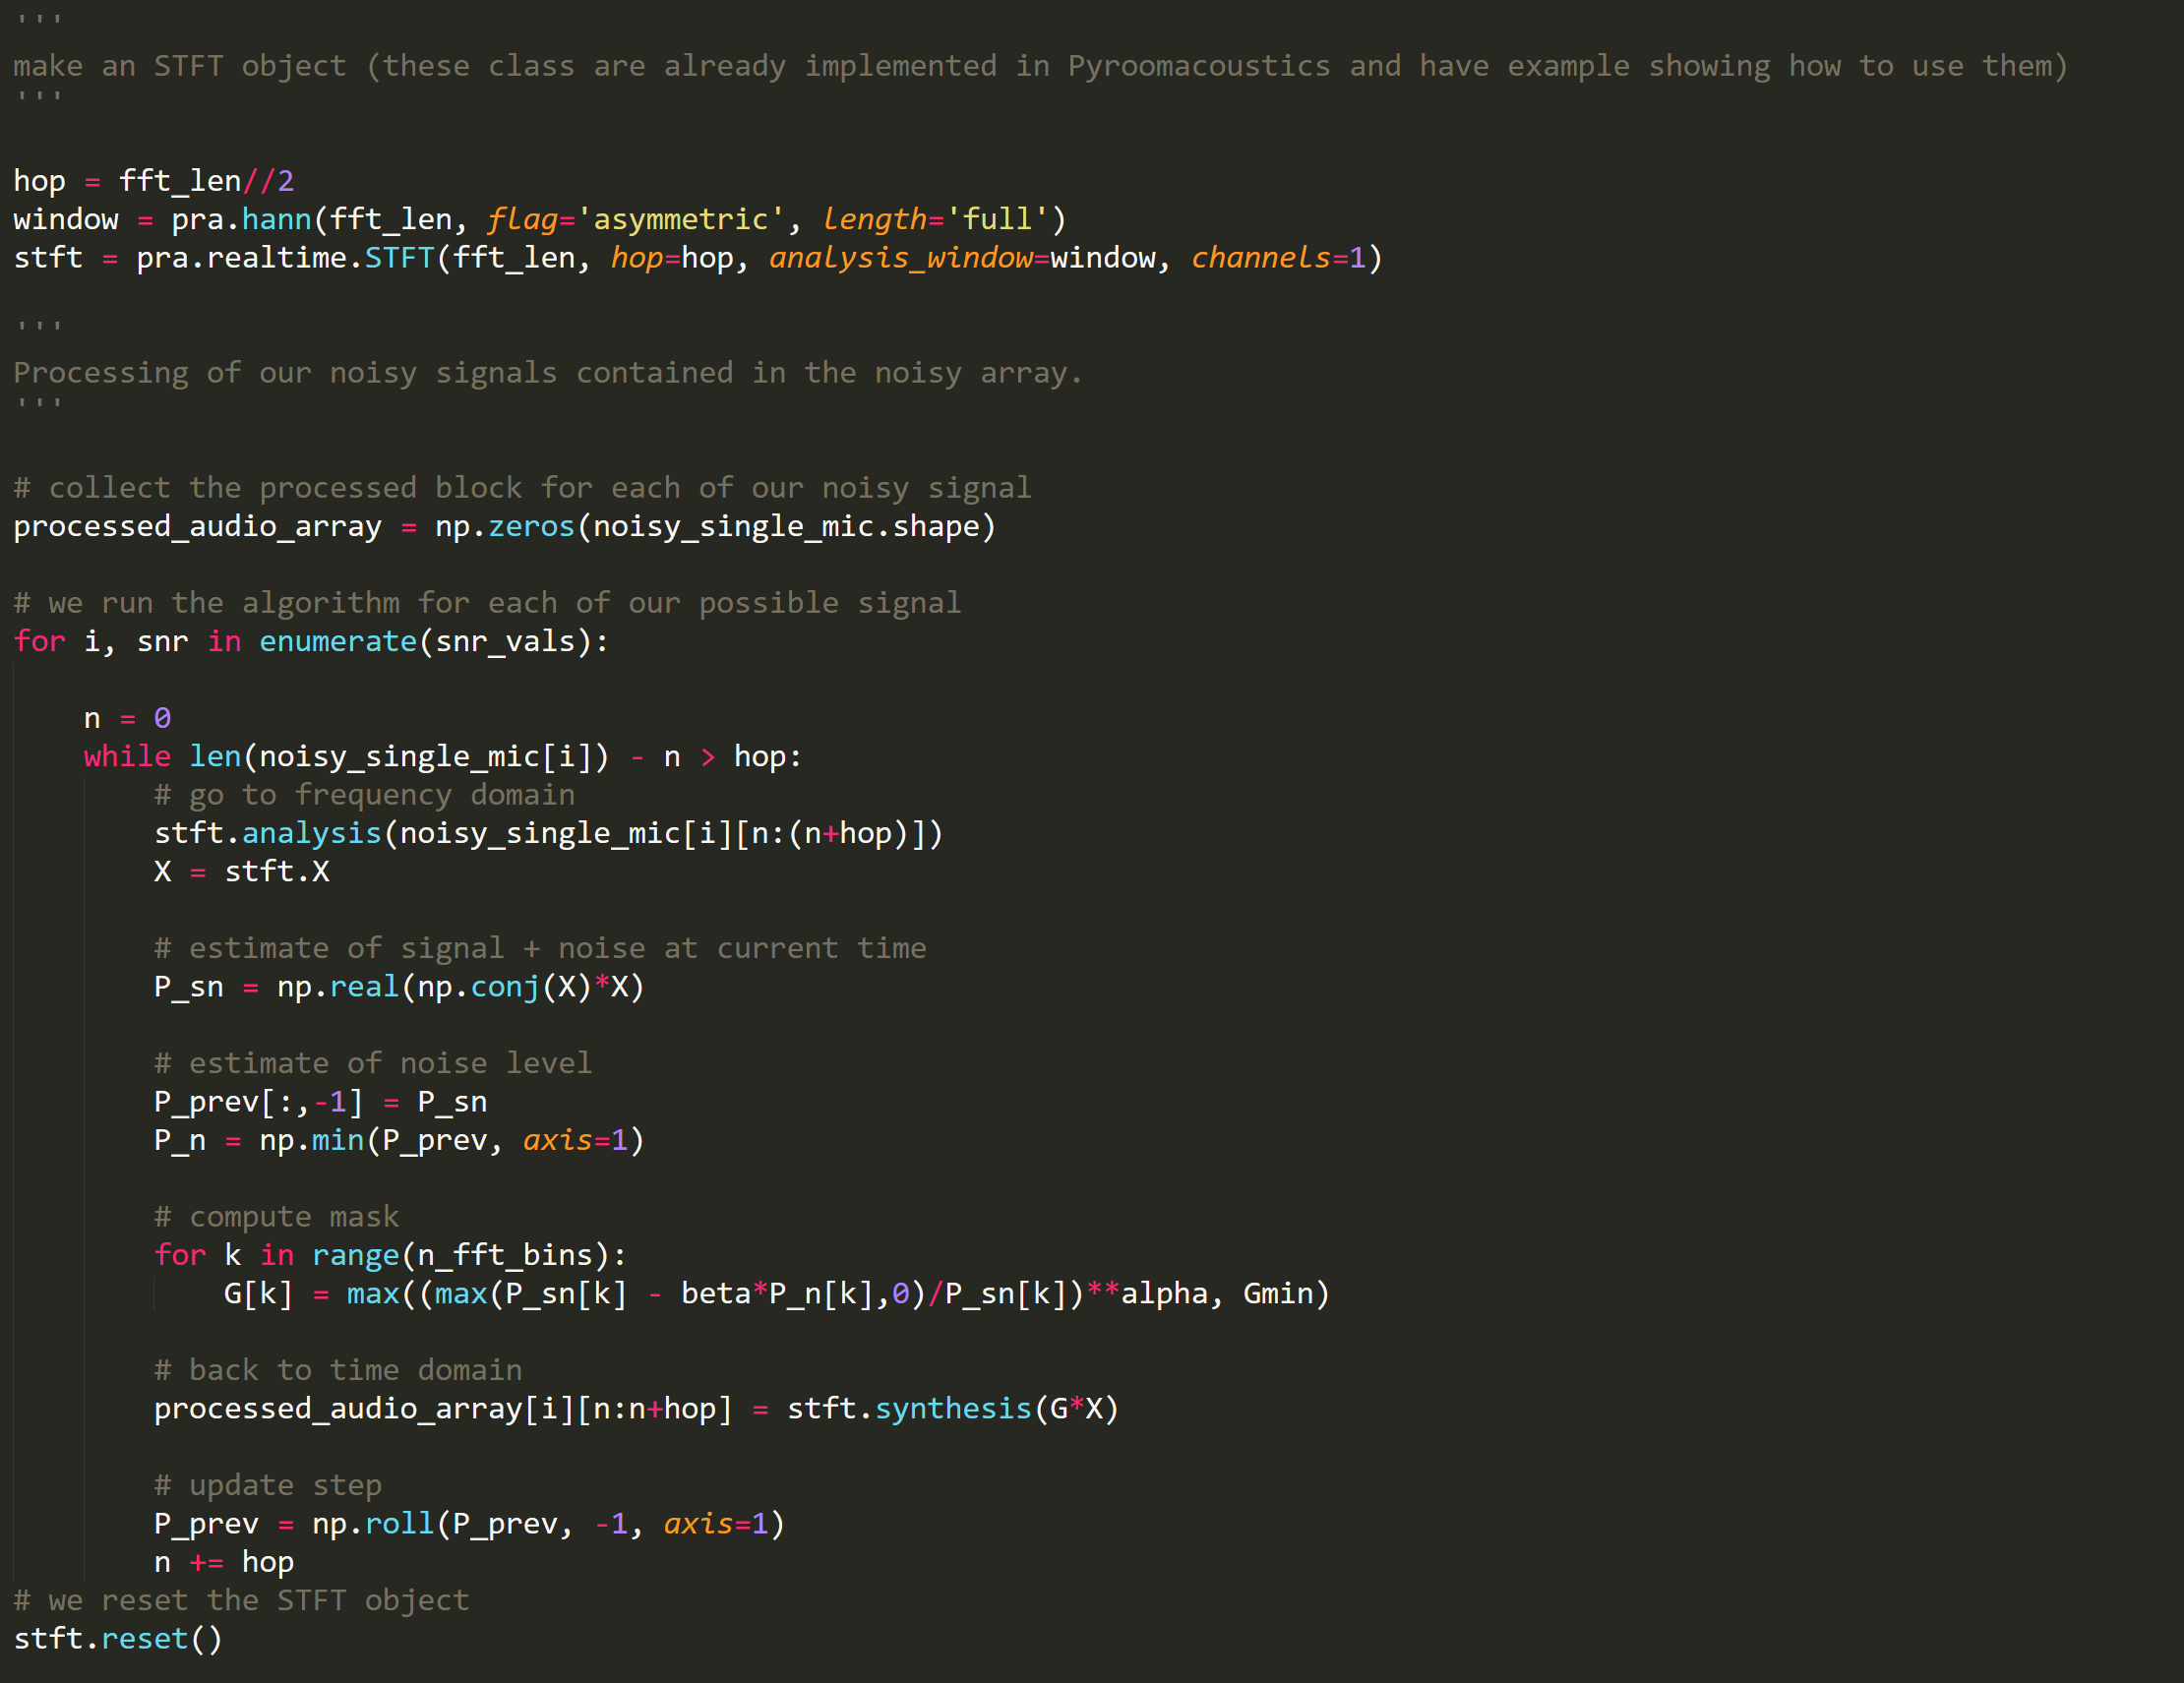
\includegraphics[width=0.7\linewidth]{rapport11}
	\caption{SCNR algorithm implemented in \textit{pyroomacoustics}}
	\label{fig:rapport11}
\end{figure}

\chapter{Results}
\hspace*{0.6cm}
In this section we will look at the performance of the two algorithms when we try to labelled processed sound. First we will talk about the SNCR and then about the DAS.
\section{Analyse improvement of Single Noise Channel Removal}
\hspace*{0.6cm}
We first tried the SNCR algorithm in a script called:\\ ``analyze\_improvement\_of\_single\_noise\_channel\_removal\_fulldata" avaible in \textit{pyroomacoustics}. We ran it for subset of size 25 in the GoogleSpeechCommands dataset and for all the word that the TenserFlow neural network can recognize. This means we have created 1750 samples per word and 25 samples per SNR for a given word.\\
We obtained the following result:
\begin{figure}[h!]
	\centering
	\begin{subfigure}{.32\textwidth}
		\centering
		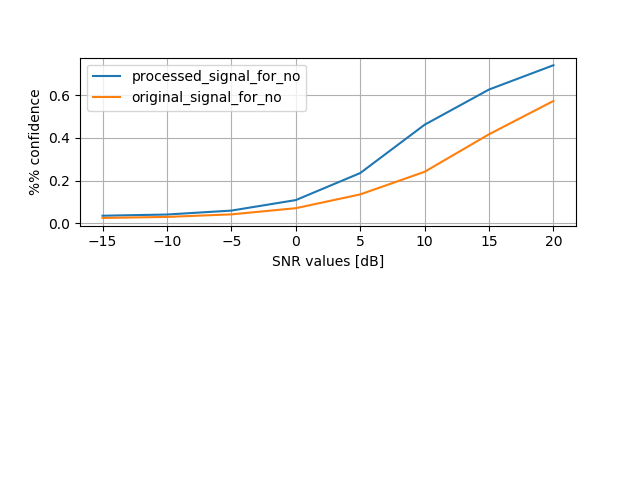
\includegraphics[width=1.2\linewidth]{rapport_no_single_noise_channel_removal}
		\caption{classification of the word no}
		\label{fig:sub3}
	\end{subfigure}%
	\begin{subfigure}{.32\textwidth}
		\centering
		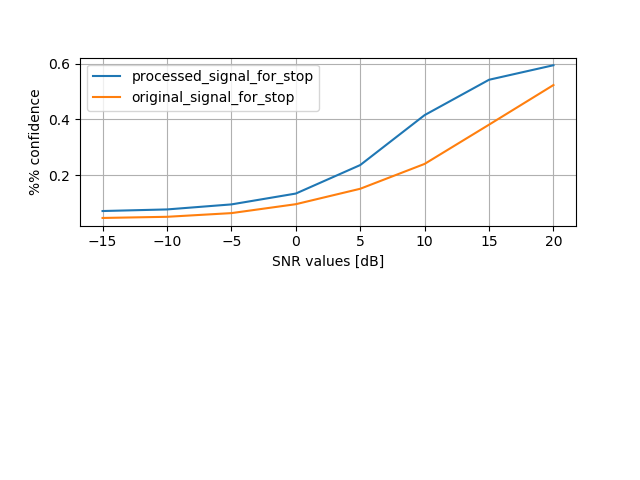
\includegraphics[width=1.2\linewidth]{rapport_stop_single_noise_channel_removal}
		\caption{classification of the word stop}
		\label{fig:sub4}
	\end{subfigure}
	\begin{subfigure}{.32\textwidth}
		\centering
		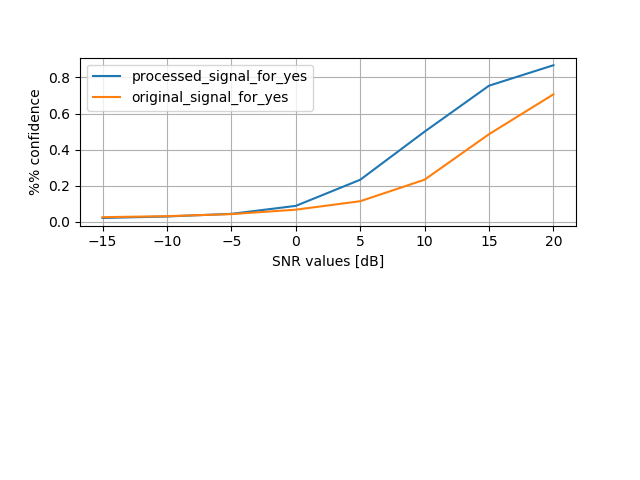
\includegraphics[width=1.2\linewidth]{rapport_yes_single_noise_channel_removal}
		\caption{classification of the word yes}
		\label{fig:sub5}
	\end{subfigure}

	\caption{classification comparison between the original noisy signal and a processed version of it using SNCR for samples of size 25}
	\label{fig:rapport12}
\end{figure}
We can see in the case of the word ``no" that the algorithm improved the recognition for low SNR (SNR that are the most plausible in real life). For example at a SNR of 10dB we have an improvement of 23$\%$ for the classification which is huge (we go from 25$\%$ of correct recognition by the model to 48$\%$). We can also see that the recognition is always higher when we are using a processed signal.
In the case of the word ``stop" we can make the same conclusion. At a SNR of 10dB we have an improvement of 19$\%$ for the classification (we go from 23$\%$ of correct recognition by the model to 42$\%$).
The result of this test is even more impressive when we are working with the word ``yes" since we have an improvement of the classification of 29$\%$ at a SNR of 10dB (we go from 23$\%$ of correct recognition by the model to 52$\%$).
We can conclude that the SNCR is a good algorithm for cleaning the data before giving it to a classifier. The improvement for low SNR are always close or above 20$\%$. But we can't say this is perfect. Even if the algorithm is quick, we can see that we don't achieve more that 50$\%$ of correctness in a majority of the case  for low SNR. This is not that good if we want for example to use this algorithm for a vocal recognition system.
\section{Analyse improvement of Beamforming}
\chapter{Conclusion}
\section{Where are we now?}
\hspace*{0.6cm}
At the end of this project we were able to add a wrapper to Google's Speech Commands Dataset, to add utilities for augmenting  datasets and to test the efficiency of processing algorithm for improving the recognition's quality of a system. We have seen that SNCR is working quite well for what we are doing right now but we can surely do much better (but we will talk about this at the end).\todo{beamforming}\\ 
All the scripts we have done are now available on the GitHub of \textit{pyroomacoustics} at the address \url{https://github.com/LCAV/pyroomacoustics}. 

\section{What's next?}
In the future and for the improvement of the \textit{pyroomacoustics} library, other students could test and implement other signal processing algorithm (for example just test the other beamforming algorithms already available in the package). They could also create new wrapper for other datasets. Then they could also create a new dataset from scratch for \textit{pyroomacoustics} which could help user to test their algorithms in the best condition possible (also it could be quite fun to record sound). Finally, they could try to find other machine learning model with better accuracy to improve what we have right now in \textit{pyroomacoustics}.
\chapter{Bibliography}
1) arXiv:1710.04196v1 [cs.SD],
	Robin Scheibler, Eric Bezzam,
		Ivan Dokmanic, \textit{"Pyroomacoustics: a python package for audio room simulation and array processing algorithms"},
	Ecole Polytechnique F�d�rale de Lausanne (EPFL),
		University of Illinois Urbana-Champaign, USA,
	11 Oct 2017
\\
\\
2) TensorFlow,
	\textit{Simple Audio Recognition},
	13 January 2018,
	\url{https://www.tensorflow.org/versions/master/tutorials/audio_recognition}
\\
\\
3) Pete Warden, Software Engineer, Google Brain Team, 
   Google AI Blog,
   \textit{Launching the Speech Command Dataset}
   24 August 2017
   \url{https://ai.googleblog.com/2017/08/launching-speech-commands-dataset.html}
\\
\\
4) J�rgen Grythe, 
	\textit{Array gain and reduction of self-noise}, 
	Norsonic AS, Oslo, Norway,
	2016
\\
\\
5) Christof Faller and Dirk Schr�der,
	\textit{Audio Signal Processing and Virtual Acoustics},
	9 September 2015,
\\
\\
6) 10.1109/ICASSP.2015.7178030,
	Robin Scheibler, Ivan Dokmanic, and Martin Vetterli, 
	\textit{Raking Echoes in the time domain }, 
	School of Computer and Communication Sciences
	Ecole Poly technique Federale de Lausanne (EPFL), CH-IOI5 Lausanne, Switzerland,
	2015

\end{document}